\section{1st Model}
\label{sec:Model}

In an effort to create a working trust model iteratively, we will start by simplifying the model described by Castelfranchi and Falcone \cite{Castelfranchi1998}, by removing the effects of outside influence in Trust representation. We also do not take into account long term considerations of the trustor's goal, reducing contextual scope to just the task being performed by the trustor. So Trust is represented by a 3-tuple:

\begin{itemize}
	\item The trustor (\textbf{X});
	\item The trustee (\textbf{Y});
	\item A task ($\bm{\tau}$) defined by the pair $(\alpha, \rho)$, where \bm{$\alpha$} is the action entrusted to the trustee, that possibly produces an outcome \bm{$\rho$}, contained in the goal of X.
\end{itemize}
\begin{equation}
TRUST(X\ Y\ \tau)
\label{eq:TrustRelation}
\end{equation}

The focus will be in properly representing a certain agent's features that contribute to a trust evaluation, as represented in Figure \ref{fig:trustee}. These features must be able to provide 2 values:
\begin{itemize}
	\item trust - a value for how much trust we have in this trustee's specific feature;
	\item certainty - the degree of how much we believe this trust assumption to be true, as factors like how many times, or how long ago, did we last affirm this belief may affect the believability of our assumptions.
\end{itemize}
\begin{figure}[hbt]
	\centering
	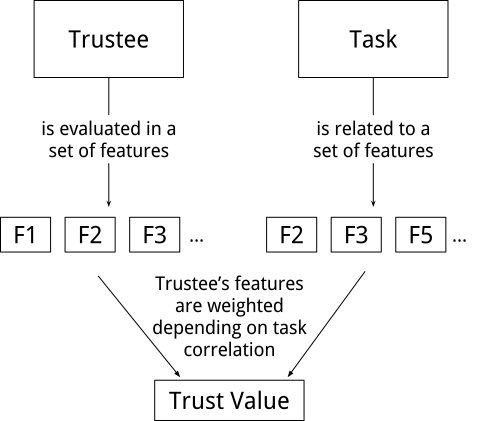
\includegraphics[height=200px]{figures/Trust_Model_Diagram.png}
	\caption{Trustee Features Representation}
	\label{fig:trustee}
\end{figure}

Trust and certainty are calculated through a collection of belief sources, which in the first version will be a history of direct contacts. The environment must be able to provide some way to access these contacts, either by a callback function or through open access to an action history. If the environment does not provide such features, a perception module, capable of checking action results, will be required.

The task is composed by a set of related features with a given weight. This represents the features most closely related to the task at hand, and their importance to he completion of the task.

\subsection{Implementation}

Implementation wise, the model will be 1st implemented by using a simple class structure, as seen in figure \ref{fig:classDiagram}. In this diagram, the main actor is the Agent, which contains a list of Trustees with features that the Agent has been able to perceive from received sources. For now the sources must be given by the simulation environment, but an interpreter should be implemented to sort out and transform the perceptions received by the environment into sources for belief features.
A simple simulation example can be performed as following:

\begin{figure}[hbt]
	\centering
	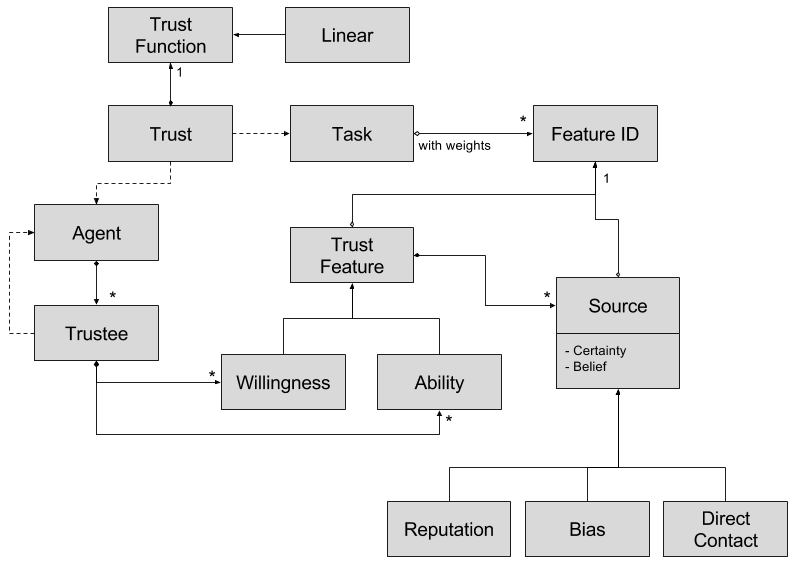
\includegraphics[height=150px]{figures/Class_Diagram.png}
	\caption{Class Diagram}
	\label{fig:classDiagram}
\end{figure}




